\subsection{Evaluating KALE}
We compare the performance of using KALE for post-training compression in figure \ref{fig:kale-not} across the five datasets and see a fairly consistent trend. When the recall set is small and the query encoders are pruned to a high degree, the impact of KALE is most visible, often driving over 50 improvements in retrieval accuracy. Additionally, using KALE allows the models to have a steady and gradual drop in recall accuracy relative to speedup instead of the sharp drop shown by the regular usage of structural pruning.  Without KALE, post-training compression causes a 20-50\% loss in retrieval accuracy. With the use of KALE, these losses are cut to 1-10\%. In practice, this allows using one or 2-layer encoder models running with CPU-based inference with minor impacts on accuracy. \\
\begin{table}[!ht]
    \centering
    \tiny
    \scalebox{0.7}{
    \begin{tabular}{|l|l|l|l|l|l|l|l|}
    \hline
        Model & Layers & KALE & MSMARCO & NQ & TriviaQA & SQUAD & SCIFACTS \\ \hline
        BERT\textsubscript{BASE} & 12 & N & 88.77\% & 85.84\% & 85.03\% & 77.16\% & 90.70\% \\ \hline
        \midrule
        BERT\textsubscript{BASE} & 6 & Y & 84.68\% & 83.68\% & 83.01\% & 69.87\% & 85.13\% \\ \hline
        $6_{kd}-6_{kd}$ & 6 & N & 88.19\% & 85.15\% & 84.96\% & 71.94\% & 91.23\% \\ \hline
        $6_{db}-6_{db}$ & 6 & N & 88.35\% & 84.74\% & 84.83\% & 71.69\% & 89.37\% \\ \hline
        $6_{kd}-3_{kd}$ & 6 & N & 86.50\% & 85.37\% & 84.04\% & 70.89\% & 89.20\% \\ \hline
        \midrule
        BERT\textsubscript{BASE} & 3 & Y & 82.11\% & 81.14\% & 81.67\% & 64.37\% & 82.57\% \\ \hline
        $3_{kd}-3_{kd}$ & 3 & N & 86.13\% & 83.66\% & 84.11\% & 71.98\% & 89.40\% \\ \hline
        $3_{kd}-6_{kd}$ & 3 & N & 84.79\% & 85.76\% & 83.91\% & 67.85\% & 88.63\% \\ \hline
        $6_{kd}-3_{kd}$ & 3 & Y & 82.95\% & 83.43\% & 82.33\% & 63.77\% & 90.37\% \\ \hline
        $6_{kd}-6_{kd}$ & 3 & Y & 86.75\% & 80.78\% & 83.48\% & 64.14\% & 91.70\% \\ \hline
        \midrule
        BERT\textsubscript{BASE} & 2 & Y & 81.96\% & 81.94\% & 81.23\% & 67.00\% & 82.57\% \\ \hline
        $3_{kd}-3_{kd}$ & 2 & Y & 84.23\% & 82.71\% & 83.02\% & 67.02\% & 91.33\% \\ \hline
        $3_{kd}-6_{kd}$ & 2 & Y & 85.57\% & 84.27\% & 82.90\% & 62.75\% & 88.37\% \\ \hline
        $6_{kd}-3_{kd}$ & 2 & Y & 83.24\% & 83.02\% & 82.13\% & 62.52\% & 89.93\% \\ \hline
        $6_{kd}-6_{kd}$ & 2 & Y & 85.77\% & 80.39\% & 83.32\% & 52.74\% & 91.93\% \\ \hline 
        \midrule
        BERT\textsubscript{BASE} & 1 & Y & 48.05\% & 71.33\% & 75.40\% & 51.39\% & 66.83\% \\ \hline
        $3_{kd}-3_{kd}$ & 1 & Y & 66.69\% & 77.17\% & 80.82\% & 55.62\% & 76.03\% \\ \hline
        $3_{kd}-6_{kd}$ & 1 & Y & 72.13\% & 79.81\% & 80.23\% & 52.26\% & 78.67\% \\ \hline
        $6_{kd}-3_{kd}$ & 1 & Y & 71.26\% & 76.57\% & 78.65\% & 50.88\% & 77.07\% \\ \hline
        $6_{kd}-6_{kd}$ & 1 & Y & 70.70\% & 74.71\% & 80.31\% & 52.74\% & 77.89\% \\ \hline
    \end{tabular}}
    \caption{Impact of model asymmetry and use of KALE for structural pruning on the Retrieval at 100 accuracies across various datasets. }
    \label{tab:kale+asym-100}
\end{table}
We also notice a surprising performance improvement between 3 and 2-layer query encoders with and without KALE. We believe this shows the phenomena studied elsewhere: the first and last layers do most of the work \cite{Oh2022DontJA}. 
\subsection{Aiding Asymmetry with KALE}
Seeking to optimize compression further, we combine KALE with asymmetrical finetuning and evaluate the results similarly to our earlier experiments. Results on the impact of KALE and asymmetry on the five datasets on the recall accuracy at 100 can be found in table \ref{tab:kale+asym-100} where $3_{kd}-6_{kd}$ denotes a three-layer query encoder and six-layer document encoder, $3_{kd}-3_{kd}$ denotes dual three layer encoders. Full results and metrics for each task can be found in the appendix section \ref{sec:kale-asym-full}. \\
\begin{figure}[!htb]
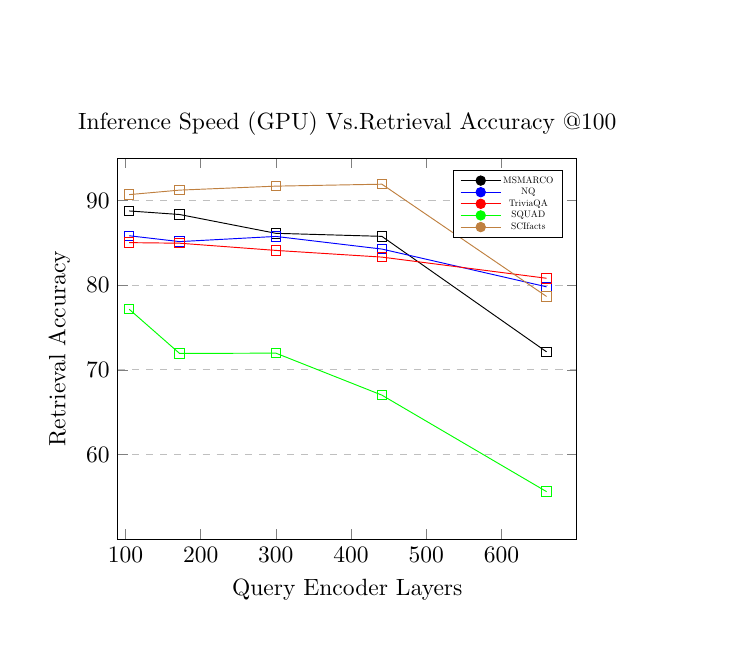
\begin{tikzpicture}
\scalebox{0.85}{
\begin{axis}[
    title={Inference Speed (GPU) Vs.Retrieval Accuracy @100   },
    xlabel={Query Encoder Layers},
    ylabel={Retrieval Accuracy},
    xmin=90, xmax=700,
    ymin=50 , ymax=95,
    xtick={100, 200, 300,400,500,600},
    ytick={60,70,80,90},
    legend pos=north east,
    ymajorgrids=true,
    grid style=dashed,
    legend style={nodes={scale=0.4, transform shape}}, 
    legend image post style={mark=*}
]
\addplot[
    color=black,
    mark=square,
    ]
    coordinates {
    (105, 88.77) (172,88.35) (300,86.13) (441, 85.77) (660, 72.13)
    };
\addplot[
    color=blue,
    mark=square,
    ]
    coordinates {
    (105, 85.84) (172,85.15) (300,85.76) (441, 84.27) (660, 79.81)
    };
\addplot[
    color=red,
    mark=square,
    ]
    coordinates {
    (105, 85.03) (172,84.96) (300,84.11) (441, 83.32) (660, 80.82)
    };
\addplot[
    color=green,
    mark=square,
    ]
    coordinates {
    (105,77.16) (172,71.94) (300,71.98) (441,67.02) (660, 55.62)
    };
\addplot[
    color=brown,
    mark=square,
    ]
    coordinates {
    (105, 90.7) (172,91.23) (300,91.7) (441, 91.93) (660, 78.67)
    };

\legend{MSMARCO, NQ, TriviaQA, SQUAD, SCIfacts }
 \end{axis}}

\end{tikzpicture}
    \centering
    \caption{The impact on retrieval accuracy of the best combinations of asymmetrical training and KALE across the NQ, MSMARCO, TriviaQA, SQUAD, and SCIfacts retrieval datasets}
    \label{fig:speed-vs-acc}
\end{figure}
First, it is immediately observable that post-training compression via KALE performs worse than models natively designed for that size. We believe this is due to the convergence of the KALE models to have \textit{some distance} from the uncompressed model because of dropout. We experimented with not using dropout in KALE, but model performance quickly suffered. \\
Looking at the best retrieval accuracy vs. the model speedups shown in figure \ref{fig:speed-vs-acc}, we can see a substantial variation in the impact of compression across datasets. In tasks like SCIfacts, it is possible to get over 4x speedup while improving accuracy, while on tasks like SQuAD, even minor speedups lead to major losses in accuracy. We believe this variation is driven by the relative difficulty of each dataset, where easier tasks are more compressible than harder tasks. \\
We believe these variations in results highlight the utility of post-training compression methods like KALE. Given the task variability in the impact of compression, iteration speed and cost are essential to effectively tuning model inference speed and accuracy. 
\section{Conclusion and Future Work}
In this work, we have demonstrated how the use of asymmetry between the query and document encoders in bi-encoder models can be leveraged for improved inference efficiencies across CPUs and GPUs. Using our post-training compression framework, KALE, we can compress models up to 6x with little loss in accuracy. Compressing models without regenerating the document index or the document encoder makes it practical to have many query encoders tailored to each use case's latency needs. \\
In the future, we wish to study how asymmetry in retrieval can be implemented with models which are widely different and may have different hidden sizes, such as using MiniLM for the query model and RoBERTA-Large for the document model. 